%\documentclass[serif,14pt,color=usenames,dvipsnames,aspectratio=169]{beamer}
\documentclass[serif,14pt,color=usenames,dvipsnames]{beamer}
\usepackage{elastic}
\usepackage{dashbox}
\usepackage{hyperref}

\usetikzlibrary{backgrounds}
\newcommand{\mystar}{\small $\bigstar$}

\title{{\Large Digital Humanities}\\survival kit}
\author{André Santos, \href{mailto:afs@inesctec.pt}{afs@inesctec.pt}}


\begin{document}

\begin{frame}
\maketitle
\end{frame}



% photoscan
% garageband
% encryption
  % wikileaks
% evernote
% grammarly
% afterlight
% qr codes



\begin{frame}{Smartphones}
  \begin{columns}
    \column{0.48\textwidth}
    \begin{itemize}
      \item phone book
      \item flashlight
      \item camera
      \item video camera
      \item sound recorder
      \item clock
      \item alarm clock
      \item GPS
      \item calendar
    \end{itemize}
    \column{0.48\textwidth}
    \begin{itemize}
      \item dictionary
      \item grocery list
      \item news
      \item music player
      \item movie theater
      \item ebook reader
      \item compass
      \item credit card
      \item 
    \end{itemize}
  \end{columns}
\end{frame}

\begin{frame}{PhotoScan}
  \centering

  \begin{figure}
  
\includegraphics[width=0.3\linewidth]{imgs/photoscan2}
  \end{figure}
  \vspace{0.5cm}
  \href{https://google.com/photos/scan/}{google.com/photos/scan/}
\end{frame}

\begin{frame}{Photo Exif Editor Pro}
  \centering

  \begin{figure}
  
\includegraphics[width=0.3\linewidth]{imgs/exif}
  \end{figure}

  \href{https://play.google.com/store/apps/details?id=net.xnano.android.photoexifeditor}{Google
  Play \beamergotobutton{Link}}
\end{frame}

\begin{frame}{Voice Recorder}

\end{frame}

\begin{frame}{Noise removal}
\end{frame}

\begin{frame}{External mic}
\begin{columns}
  \column{0.3\textwidth}
    
\includegraphics[width=\linewidth]{imgs/phone}
  \column{0.3\textwidth}
    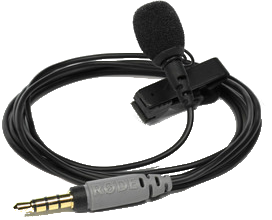
\includegraphics[width=\linewidth]{imgs/mic}
  \column{0.3\textwidth}
    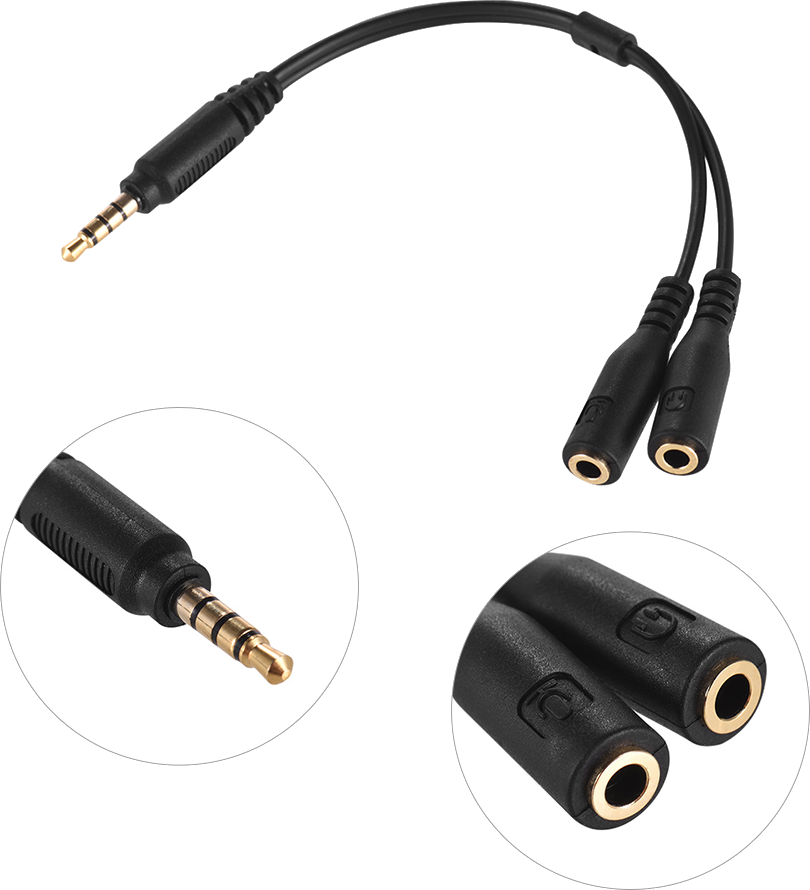
\includegraphics[width=\linewidth]{imgs/trrs}
\end{columns}
\end{frame}


\begin{frame}{External mic (iPhone)}
  \centering
  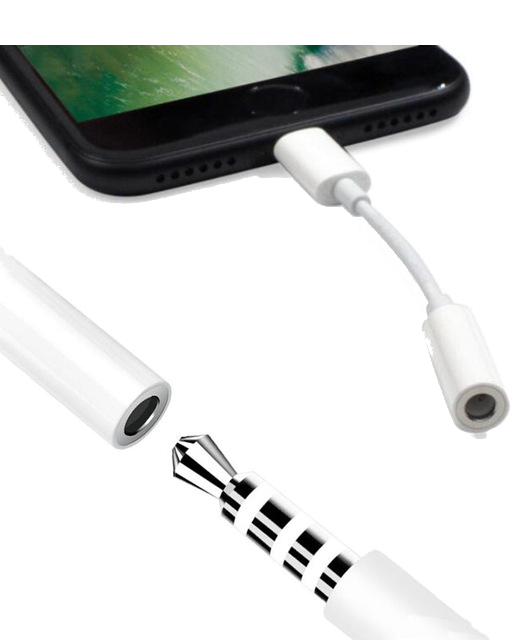
\includegraphics[width=0.4\linewidth]{imgs/35mm}
\end{frame}

\begin{frame}{Smart Doc Scanner}
  \centering

  \begin{figure}
  
\includegraphics[width=0.3\linewidth]{imgs/sds}
  \end{figure}

  \href{https://www.youtube.com/watch?v=zAcMvZpTeBo}{YouTube \beamergotobutton{Link}}

  \href{https://play.google.com/store/apps/details?id=com.mobilicy.docscanner}{Google
  Play \beamergotobutton{Link}}
\end{frame}

\begin{frame}{PhotoSphere}

  \begin{itemize}
    \item Take multiple pictures
    \item Merge them together
    \item Allow to pan and zoom
  \end{itemize}

  \centering

  \begin{figure}
  
\includegraphics[width=0.3\linewidth]{imgs/photosphere}
  \end{figure}

  \href{https://www.youtube.com/watch?v=NPs3eIiWRaw}{YouTube \beamergotobutton{Link}}

  \href{https://g.co/photosphere}{g.co/photosphere \beamergotobutton{Link}}

\end{frame}

\begin{frame}{Version control}

\end{frame}

\begin{frame}{Secure messaging}
\end{frame}

\begin{frame}{Bigvu}
https://www.youtube.com/watch?time_continue=2&v=-yqQnW5s70E
https://play.google.com/store/apps/details?id=bigvu.com.reporter
\end{frame}

\begin{frame}{Evernote}
\end{frame}

\begin{frame}{Automatic Call Recorder Pro}
\end{frame}

\end{document}


\begin{frame}{New students}
  \begin{block}{Fill the form}
  \url{https://goo.gl/7DnCxC}
  \end{block}
  \begin{block}{Repositories}
    \begin{itemize}
    \item \url{github.com/andrefs/spln-docs}
    \item \url{github.com/andrefs/spln-2018-i}
    \end{itemize}
  \end{block}
\end{frame}

\begin{frame}{Unix philosophy}
\begin{itemize}
  \item Write programs that \emph{do one thing} and do it well.
  \item Write programs to \emph{work together}.
  \item Write programs to \emph{handle text streams}, because that is a universal interface.
  \begin{flushright}
    \textit{Peter H. Salus, 1994}
  \end{flushright}
\end{itemize}
\end{frame}

\begin{frame}{Unix filters}
  \begin{itemize}
    \item software program that takes an input and produces an output
    \item can be used in a stream operation
    \item can be mixed and matched to create complex operations
  \end{itemize}
\end{frame}

\begin{frame}[fragile]{Filter example: \texttt{tail}}
  \begin{itemize}
    \item input from STDIN or files (arguments)
    \begin{minted}{bash}
find | tail
tail my_large_file.txt
    \end{minted}
    \item output to STDOUT (can be redirected)
    \begin{minted}{bash}
tail my_large_file | nl
tail my_large_file > last_lines.txt
    \end{minted}
    \item behavior modified with command line arguments
    \begin{minted}{bash}
tail -n 20 my_large_file # show 20 lines
    \end{minted}
  \end{itemize}
\end{frame}

\begin{frame}{Unix filters}
\begin{itemize}
  \item \emph{head}: first lines
  \item \emph{tail}: last lines
  \item \emph{cut}: remove columns
  \item \emph{paste}: merge lines of files
  \item \emph{nl}: number lines
  \item \emph{wc}: count lines, words and chars
  \item \emph{grep}: filter by pattern
  \item \emph{cat}: (concat and) print
\end{itemize}
\end{frame}

\begin{frame}{Unix filters}
\begin{itemize}
  \item \emph{tr}: translate or delete characters
  \item \emph{sed}: stream editor for filtering and transforming text
  \item \emph{awk}: pattern scanning and processing language
  \item \emph{perl}: Perl (can be used like awk)

  \item \emph{sort}: sort lines of text files
  \item \emph{uniq}: report or omit repeated lines
  \item \emph{tee}: read from standard input and write to standard output and files
\end{itemize}
\end{frame}

\begin{frame}[fragile]{Filter composition}
\begin{itemize}
  \item Calc. the most used bash commands
\begin{minted}{bash}
history \
  | awk '{a[$4]++}END{for(i in a){print a[i] "\t" i}}' \
  | sort -rn \
  | head
\end{minted}
  \item Sort lines by the number of occurrences (desc)
\begin{minted}{bash}
sort | uniq -c | sort -nr
\end{minted}
  \item Generate 100 random characters
\begin{minted}{bash}
cat /dev/urandom \
  | tr -dc "0-9a-zA-Z!@#$%^&*_+-" \
  | head -c 100
\end{minted}
\end{itemize}
\end{frame}

\begin{frame}[fragile]{System calls}
\begin{minted}{python}
import subprocess

exit_code = subprocess.call(["ls", "-l"])

# returns output as byte string
output = subprocess.check_output('ifconfig')

# using decode() function to convert byte string to string
print(returned_output.decode("utf-8"))
\end{minted}
\end{frame}

\begin{frame}[fragile]{\large Unix filter with Python}
  \vspace{-0.5cm}
\begin{minted}{Python}
import getopt
import sys

options, remainder = getopt.getopt(sys.argv[1:], 'abc:', \
  ['output=', 'verbose', 'version='])
dict_opts = dict(options)

# input from STDIN or file
if remainder:
  input = open(remainder[0])
else:
  input = sys.stdin


# output to STDOUT or file
out = dict_opts.get('--output', None)
if out:
  output = open(out, 'w+')
else:
  output = sys.stdout

output.write("".join(input.readlines()))
\end{minted}
\end{frame}


\begin{frame}[fragile]{Unix filter (simpler version)}
\begin{minted}{Python}
import fileinput, getopt, sys, re
opts, args = getopt.getopt(sys.argv[1:], "d")

for line in fileinput.input(args):
  line = line.strip()
   # ...
\end{minted}
\end{frame}

\begin{frame}{Exercises}
\begin{enumerate}
  \item Write a sequence of Unix filters to print lines 40 to 50 of a
    file
  \item Write a Python script which does the same thing by using
    system calls
  \item Rewrite the script without using system calls
\end{enumerate}
\end{frame}


\begin{frame}{Regular expressions}
  \begin{block}{~}
    \textbf{RegEx} are a language for specifying text search strings.
  \end{block}
  \begin{itemize}
    \item They are used to specify \textit{patterns} to be matched
      against \textit{strings}.
    \item Tipically used in word processors and text editors, search
      engines and text processing utilities.
    \item Also, in programming languages:
      \begin{itemize}
        \item Perl, Java \texttt{java.util.regex}, \emph{Python \texttt{re}}, Ruby, \dots
      \end{itemize}
  \end{itemize}
\end{frame}

\begin{frame}[fragile]{Regular expressions}
\begin{minted}{python}
import re

string = 'This is my string'

re.findall(r'my', string)     # ['my']
re.sub(r'my', 'your', string) # 'This is your string'
\end{minted}
\end{frame}


\begin{frame}{Regular expressions}
  \centering
  \includegraphics[width=\linewidth]{imgs/xkcd}
\end{frame}


\begin{frame}{Background}
\begin{itemize}
  \item First originated in the 1950s
  \item Regular expressions can express regular languages (languages
    accepted by deterministic finite automata)
    \item Multiple standards, most common is POSIX
\end{itemize}
\end{frame}


\begin{frame}[fragile]{Basic}
  \begin{itemize}
    \item \texttt{r'amanhã'}
\begin{minted}{python}
re.search(r'amanhã', 'O António chega amanhã.')
\end{minted}
    \item \texttt{r'gat.'}
\begin{minted}{python}
re.search(r'sac.', 'O João leva os livros numa saca.')
\end{minted}

  \end{itemize}
\end{frame}

\begin{frame}[fragile]{Quantification}
  \begin{itemize}
    \item \texttt{r'golo'}
\begin{minted}{python}
re.search(r'golo', 'Ronaldo chuta e... golo!!!')
\end{minted}
    \item \texttt{r'goloo?'}
\begin{minted}{python}
re.search(r'goloo?', 'Ronaldo chuta e... goloo!!!')
\end{minted}
  \end{itemize}
\end{frame}


\begin{frame}[fragile]{Quantification}
  \begin{itemize}
    \item \texttt{r'golo+'}
\begin{minted}{python}
re.search(r'golo+', 'Ronaldo chuta e... golooooooo!!!')
\end{minted}
    \item \texttt{r'goloo*'}
\begin{minted}{python}
re.search(r'goloo*', 'Ronaldo chuta e... golo!!!')
\end{minted}
    \item \texttt{r'golo\{2,5\}'}
\begin{minted}{python}
re.search(r'golo{2,5}', 'Ronaldo chuta e... golooo!!!')
\end{minted}
  \end{itemize}
\end{frame}

\begin{frame}[fragile]{Grouping}
  \begin{itemize}
    \item 'aldeão'
      \pause
    \begin{itemize}
    \item aldeãos, aldeões, aldeães
    \end{itemize}
    \pause
\begin{minted}{python}
re.search(r'alde(ão|ãe|õe)s', \
  'Os aldeões fizeram uma festa na aldeia.')
\end{minted}
  \end{itemize}
\end{frame}

\begin{frame}[fragile]{Disjunction and intervals}
  \begin{itemize}
    \item \verb![AEIOU]!
    \item \verb![0123456789]!
    \item \verb!alun[oa]!
    \pause
    \item \verb![A-Z]!
    \item \verb![0-9]!
    \item \verb![0-9A-F]!
    \pause
    \item \verb![^aeiou]!
  \end{itemize}

\end{frame}

\begin{frame}[fragile]{Character classes}
  \begin{itemize}
    \item \verb!\d! (digit)
      \begin{itemize}
        \item \verb!\D! (not \verb!\d!)
      \end{itemize}
    \item \verb!\w! (letter, digit or underscore)
      \begin{itemize}
        \item \verb!\W! (not \verb!\w!)
      \end{itemize}
    \item \verb!\s! (whitespace)
      \begin{itemize}
        \item \verb!\S! (not whitespace)
      \end{itemize}
  \end{itemize}
\end{frame}


\begin{frame}[fragile]{Anchors}
  \begin{itemize}
    \item \verb!^! (begining of the line)
    \item \verb!$! (end of the line)
    \item \verb!\b! (word boundary)
  \end{itemize}
\end{frame}

\begin{frame}[fragile]{Capture groups}
  \begin{itemize}
    \item \verb!r'O ([A-Z][a-z]+) tem ([\w ]+)'!
\begin{minted}{python}
re.findall(r'O ([A-Z][a-z]+) tem ([\w ]+)', \
  'O Carlos tem uma mota.') # [('Carlos', 'uma mota')]
\end{minted}
    \item \verb!r'O ([A-Z][a-z]+) tem (?:[\w ]+)'! (don't capture the
      second group)
\begin{minted}{python}
re.findall(r'O ([A-Z][a-z]+) tem (?:[\w ]+)', \
  'O Carlos tem uma mota.') # ['Carlos']
\end{minted}
  \end{itemize}
\end{frame}


\begin{frame}
  \centering
  \includegraphics[width=\linewidth]{imgs/xkcd2}
\end{frame}


\begin{frame}
  \centering
  \includegraphics[height=\textheight]{imgs/regex1}
\end{frame}

\begin{frame}{Example: URLs {\fontencoding{U}\fontfamily{futs}\selectfont\char 66\relax}}
\pause
\begin{block}{~}
  \begin{columns}
    \column{0.1\linewidth}
      \centering
      \includegraphics[width=.9\linewidth]{imgs/danger1}
    \column{.83\textwidth}
      \flushleft
      \vspace{-.7cm}
      In most cases, you should not implement your own URL regex
      parser. Use 3rd party libraries such as Python's
      \fbox{\texttt{urlparse}}.
  \end{columns}
\end{block}
\pause
\begin{block}{~}
  \begin{columns}[c]
    \column{0.1\linewidth}
      \centering
      \includegraphics[width=.9\linewidth]{imgs/danger2}
    \column{.83\textwidth}
      \flushleft
      \vspace{-.7cm}
      However, it always depends on what your use case is:
      \begin{itemize}
        \item finding potential URLs in a text
        \item ensuring that a given URL is correctly formed
        \item \dots
      \end{itemize}
  \end{columns}
\end{block}
\end{frame}

\begin{frame}[fragile]{Example: URLs {\fontencoding{U}\fontfamily{futs}\selectfont\char 66\relax}}
  \begin{figure}
    \centering
    \includegraphics[width=\linewidth]{imgs/url}
  \end{figure}
  \pause
  \begin{aligndesc}{Query parameters}
    \item[Protocol]\verb!http(s?)://!
    \item[Domain name] \verb![\w-]+(\.[\w-]+)*!
    \item[Port] \verb!:\d{2,}!
    \item[Path] \verb!/[\w-\.]+(/[\w-]+)*!
    \item[Query parameters] \verb!/[\w-]+(/[\w-]+)*!
    \item[Fragment] \verb!#[\w-]+!
  \end{aligndesc}
\end{frame}

\begin{frame}[fragile]{Example: URLs {\fontencoding{U}\fontfamily{futs}\selectfont\char 66\relax}}

\begin{minted}{python}
import re

protocol         = r'http(s?)://'
domain_name      = r'[\w-]+(\.[\w-]+)*'
port             = r':\d{2,}'
path             = r'/[\w\.-]+(/[\w\.-]+)*'
query_parameters = r'\?[\w-]+=[\w-]+(&[\w-]+=[\w-]+)*'
fragment         = r'#[\w-]+'

url_re = protocol + domain_name + port + path + \
  query_parameters + fragment

text = 'https://en.wikipedia.org:80/w/index.php' + \
  '?title=Regular_expression#Basic_concepts'

re.search(url_re, text)
\end{minted}
\end{frame}


\begin{frame}[fragile]{RegEx functions}
\begin{itemize}
  \item \texttt{re.search}
  \item \texttt{re.match}
  \item \texttt{re.findall}
  \item \texttt{re.sub}
\end{itemize}
\end{frame}

\begin{frame}[allowframebreaks]{Exercises II}
  Define regular expressions to match strings that:
\begin{enumerate}
  \item have a 't'
  \item have a 't' or a 'T'
  \item have a letter (and how many)
  \item have a digit
  \item have a decimal number
  \item have a length higher than 3 characters
  \item have an 'M' but not an 'm'
  \item have a character repeated twice
  \item have only one character repeated many times
  \item put all words between \texttt{\{ \}}
\end{enumerate}
\end{frame}

\begin{frame}[allowframebreaks]{Exercises III}
  Create a file with some text (copy something from a news website,
  for example). Write Python scripts which receive text as input and:
\begin{enumerate}
\item Outputs the text with marks on the begining
  of sentences (for example, '\#\#\# ')
\item Finds and prints proper names
\end{enumerate}
\end{frame}


\begin{frame}{Practical assignment \#1}
\begin{itemize}
  \item Choose 1 of the 3 options (A, B or C)
  \item Groups of 2 or 3 elements
  \item Submission date: October 11, 2018
  \item Web address for submission will be announced in Blackboard
\end{itemize}
\end{frame}

\begin{frame}[allowframebreaks]{Practical assignment \#1}
\begin{itemize}
  \item \emph{A)} Write a program to convert text to ASCII (remove accents).
    It should work as a Unix filter
  \item \emph{B)} Given a file with a list of words (one word per line), find
    which words can be written as a sequence of chemical symbols (ex:
    "bacon" = Ba + Co + N)
  \item \emph{C)} Write a program which, given a
    \emph{large} text with accents -- ``O João amanhã vai andar a pé
    (\dots)'' -- and a text with no accents -- ``O Ze tem um cao castanho
    (\dots)'' -- adds the accents to the second text.
\end{itemize}
\end{frame}


\begin{frame}{Practical assignment \#1}
  \centering

  Files and descriptions available at the 
  \href{https://github.com/andrefs/spln-2018-i/tree/master/data/assignments/1}{\emph{SPLN
  2018 repository}}.
\end{frame}


% \begin{frame}{References}
% \end{frame}


